\documentclass[12pt]{article}

\usepackage[utf8x]{inputenc}
\usepackage[spanish]{babel}

% COMENTARIOS DE MÁS DE UNA LÍNEA
\usepackage{comment}
% BIBLIOGRAFIA
\usepackage{natbib}
\bibliographystyle{apalike}
\usepackage{multirow}
\usepackage{geometry}
\usepackage[hyphens]{url}
\renewcommand{\bibsection}{}
% COLORES LETRA
\usepackage{xcolor}
% LO DE PORTADA
\usepackage{amssymb,amsmath,amsthm,amsfonts}
\usepackage{calc}
\usepackage{graphicx}
\usepackage{subfigure}
%\usepackage{natbib}
\usepackage{url}
\usepackage[utf8x]{inputenc}
\usepackage{amsmath}
\usepackage{graphicx}
\usepackage{gensymb} %Símbolo de grado -> \degree
\usepackage{float}
\usepackage{caption}
\graphicspath{{Imágenes/}}
\usepackage{hyperref}
\usepackage{parskip}
\usepackage{fancyhdr}
\usepackage{vmargin}
\setmarginsrb{3 cm}{2.5 cm}{3 cm}{2.5 cm}{1 cm}{1.5 cm}{1 cm}{1.5 cm}
\title{Visión Artificial}					% Titulo
\author{Lola Conde Herrera}					% Autor
\date{\today}						% Fecha
\usepackage{hyperref}
\hypersetup{colorlinks=true, urlcolor=magenta, linkcolor=black}
\urlstyle{same}
\makeatletter
\let\thetitle\@title
\let\theauthor\@author
\let\thedate\@date
\makeatother

\pagestyle{fancy}
\fancyhf{}
\rhead{\theauthor}
\lhead{\thetitle}
\cfoot{\thepage}

\begin{document}

%%%%%%%%%%%%%%%%%%%%%%%%%%%%%%%%%%%%%%%%%%%%%%%%%%%%%%%%%%%%%%%%%%%%%%%%%%%%%%%%%%%%%%%%%

\begin{titlepage}
	\centering
    \vspace*{0.0 cm}
    
\includegraphics[scale = 0.13]{logoUMU.png}\\[1.0 cm]	% Logo Universidad
    \textsc{MEMORIA DE VIA:\\ SOLUCIONES A LOS EJERCICIOS PROPUESTOS}\\[1.0 cm]	% Nombre Universidad
	\rule{\linewidth}{0.2 mm} \\[0.4 cm]
	{ \huge \bfseries \thetitle}\\
	\rule{\linewidth}{0.2 mm} \\[1.5 cm]

    \begin{minipage}{0.4\textwidth}
		\begin{center} \large
			\emph{Alumna:}\\
			\theauthor\linebreak
			\end{center}
	\end{minipage}\\[0.75 cm]

     \begin{minipage}{0.4\textwidth}
		\begin{center} \large
			\emph{Correo:}\\
			lola.c.h@um.es\linebreak
			\end{center}
	\end{minipage}\\[0.75 cm]

    \begin{minipage}{0.4\textwidth}
		\begin{center} \large
			\emph{Curso:}\\
			2023 - 2024\linebreak
			\end{center}
	\end{minipage}\\[0.75 cm]

    \begin{minipage}{0.4\textwidth}
		\begin{center} \large
			\emph{Convocatoria:}\\
			Junio\linebreak
			\end{center}
	\end{minipage}\\
 
	\vfill
	
\end{titlepage}

%%%%%%%%%%%%%%%%%%%%%%%%%%%%%%%%%%%%%%%%%%%%%%%%%%%%%%%%%%%%%%%%%%%%%%%%%%%%%%%%%%%%%%%%%

\tableofcontents
\pagebreak

\listoffigures
\pagebreak

\section*{Introducción}
Cada ejercicio se ha realizado en una carpeta diferente, llamada como el nombre del ejercicio. La excepción es SIFT, que se encuentra en CLASIFICADOR porque es una ampliación de este.

A su vez, se pueden observar ejemplos de funcionamiento de los ejercicios y sus tiempos de ejecución en los jupyter notebooks creados en la carpeta NOTEBOOKS. Cosas a tener en cuenta:
\begin{itemize}
    \item Estos se han creado en notebooks, de forma que se puedan observar vídeos (en la memoria no se pueden mostrar). 
    \item El ejercicio SIFT se encuentra en el notebook CLASIFICADOR. 
    \item MAPA no tiene notebook debido a que el código realizado sólo se utiliza para realizar el notebook\textit{ ejercicioMAPA.ipynb}.
\end{itemize}

\section{HANDS} \label{sec:hands}
\subsection*{Enunciado}
Amplia el ejemplo \textit{code/DL/hands/mano.py} hecho en clase para reconocer gestos simples, como por ejemplo contar el número de dedos extendidos. Haz un controlador sin contacto de varios grados de libertad que mida, al menos, distancia de la mano a la cámara y ángulo de orientación. Utilízalo para controlar alguno de tus programas.

\subsection*{Solución}
La solución está en \textit{HANDS/mano.py}.

Este programa realiza las siguientes tareas:
\subsubsection*{Mostrar una cámara}
Se captura cada fotograma, se procesa para realizar las tareas indicadas posteriormente, y se muestra.

\subsubsection*{Dibujar la palma de la mano y los dedos}

Obteniendo los puntos de la mano con la herramienta 'MediaPipe Hands`, se han realizado líneas entre el principio y el final de los dedos de la mano. 

Para la palma, primero se ha obtenido el centro de tres puntos que se encuentran en el borde de la palma, de forma que se obtiene el centro de la palma. En segundo lugar, se obtiene el radio, calculado como la distancia entre el centro y un punto que está al borde de la palma. De esta forma, se puede dibujar un círculo en la palma con el centro y radio calculados.

\subsubsection*{Calcular qué dedos hay levantados}

Para los dedos índice, corazón, anular y meñique, se ha calculado si se encuentran abiertos o cerrados usando la distancia entre el punto más bajo de la palma y el principio o el final del dedo. Si el dedo se encuentra cerrado, la distancia entre el punto más bajo de la palma y el final del dedo será menor que la distancia entre el punto más bajo de la palma y el principio del dedo. Si está abierto, es al contrario (es mayor).

Para el dedo pulgar, se ha considerado abierto si el principio del índice está más cerca del final de la mano que el final del pulgar. Si está más lejos, el dedo pulgar está cerrado.

\subsubsection*{Calcular el ángulo de orientación de la mano}

Para calcular el ángulo de orientación de la mano, se ha calculado el ángulo entre dos vectores, el vector horizontal y el vector que se encuentra entre el final de la palma y el principio del dedo corazón. El segundo vector debe formar 0 grados con el horizontal si la mano está horizontal, y si esta empieza a girar, se calcula el ángulo.

Si el principio de la palma está más a la izquierda que el principio del dedo corazón, entonces el ángulo es negativo. Esto se realiza comparando la componente x de los puntos.

\subsubsection*{Controlar una aplicación}

Si todos los dedos están levantados, se abre la aplicación, y si todos están cerrados se cierra. La condición ya estaba calculada en el cálculo de los dedos levantados.

\subsubsection*{Calcular la distancia de la mano a la cámara}

Se usa la palma de la mano para calcular la distancia. Se calcula con la fórmula siguiente:

$$\frac{\text{distancia focal} * \text{ancho de la palma en centímetros}}{\text{ancho de la palma en píxeles}} = \text{distancia a la cámara en centímetros}$$

Para calcular la distancia focal, se ha utilizado la herramienta \textit{calibrate.py}, que se puede encontrar en \href{https://github.com/albertoruiz/umucv/tree/master/code/calibrate}{el material de la asignatura}. Las fotografías tomadas para el cálculo de la distancia focal se encuentran en la carpeta \textit{HANDS/pattern}.

\subsection*{Explicación de la fórmula para el cálculo de la distancia de la mano a la cámara}

La distancia focal es la distancia (en píxeles) desde el centro del objetivo de la cámara hasta el sensor de esta. El objetivo es el lugar donde se encuentra la lente de la cámara, y el sensor es donde se proyecta la luz de la imagen para poder procesarla o almacenarla.

La distancia focal se obtiene realizando la calibración de la cámara. Su obtención es muy útil, debido a que con esta se puede calcular la distancia de la cámara a un objeto (dada una fotografía), si se sabe el tamaño de este en la realidad y en la fotografía.

Para explicar la fórmula para obtener la distancia, se necesita un objeto. Es este caso, se va a explicar con un esquema cuyo objeto es una botella:

\begin{figure}[H]
    \centering
    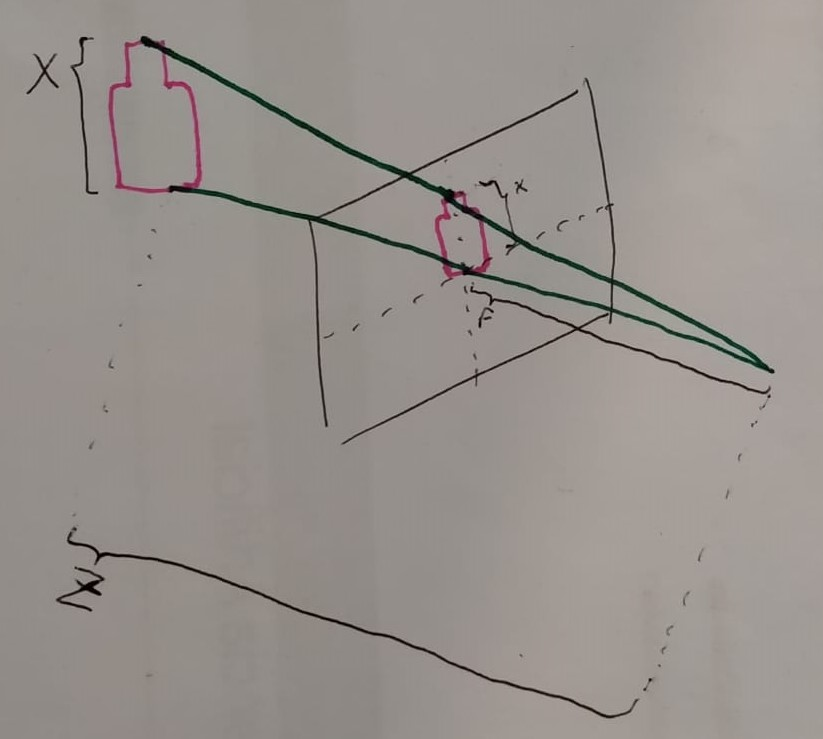
\includegraphics[scale=0.4]{Imágenes/formula1.jpeg}
    \caption{Relación entre altura de una botella en la realidad y en la foto}
    \label{fig:semana2Botella}
\end{figure}

Como se puede observar: X es la altura de la botella en el mundo real, Z es la distancia de la cámara a la botella, x es la altura de la botella en la fotografía tomada, y f es la distancia focal.

Se puede observar como se forman dos triángulos (uno con lados f y x, y otro con lados X y Z). Los triángulos se encuentran en posición de Thales, por lo que se obtiene la siguiente fórmula:

$$\frac{X}{Z}=\frac{x}{f}$$

Si se quiere obtener más información sobre el teorema de Thales, se puede observar la siguiente url: \url{https://www.superprof.es/apuntes/escolar/matematicas/geometria/basica/triangulos-en-posicion-de-thales.html}.

\subsection*{Bibliografía usada}
\href{https://github.com/google/mediapipe/blob/master/docs/solutions/hands.md}{Comprender Hand Landmark - MediaPipe}

\href{https://docs.opencv.org/3.4/d6/d6e/group__imgproc__draw.html#ga07d2f74cadcf8e305e810ce8eed13bc9}{Aprender a dibujar cuadrados}

\href{https://docs.opencv.org/3.4/d6/d6e/group__imgproc__draw.html#ga5126f47f883d730f633d74f07456c576}{Aprender a escribir texto}

\href{https://docs.opencv.org/3.4/d6/d6e/group__imgproc__draw.html#gaf10604b069374903dbd0f0488cb43670}{Aprender a dibujar círculos: cv.circle}

\href{https://docs.python.org/3/library/math.html}{Funciones de math}

\href{https://www.superprof.es/apuntes/escolar/matematicas/analitica/vectores/angulo-de-dos-vectores.html}{Ángulo entre dos vectores (para calcular la orientación de la mano)}

\href{https://github.com/albertoruiz/umucv/blob/master/notebooks/imagen.ipynb}{Material de la asignatura}

\href{https://www.sony.es/electronics/support/articles/00267921}{Entender qué es la distancia focal}

\href{https://www.blogdelfotografo.com/tipos-caracteristicas-ventajas-sensores-camaras-fotos/}{Entender qué es un sensor}

\href{https://www.superprof.es/apuntes/escolar/matematicas/geometria/basica/triangulos-en-posicion-de-thales.html}{Teorema de Thales}

También se ha usado ChatGPT para crear el programa llamado \textit{programa.py}, el cual crea una ventana. Este se utilizó para controlarlo con \textit{mano.py}, de forma que se vea la ventana abrirse y cerrarse según el gesto de la mano.

\newpage

\section{FILTROS}
\subsection*{Enunciado}

Muestra en vivo el efecto de diferentes filtros, seleccionando con el teclado el filtro deseado y modificando sus parámetros (p.ej. el nivel de suavizado) con trackbars. Aplica el filtro en un ROI para comparar el resultado con el resto de la imagen.

\subsection*{Filtros disponibles}

\subsubsection*{Blanco y negro}

En primer lugar, con el uso de la librería OpenCV se pasa a gris el color de la región de interés. Esto deja la imagen con 1 canal.

En segundo lugar, se vuelve a pasar a BGR porque este es el formato de la imagen completa. Al sobrescribir la región de interés (seleccionada) con el filtro correspondiente, lo que se escribe debe tener el mismo formato que el resto de la imagen (del fotograma).

\subsubsection*{Filtro box}

Se utiliza una función de OpenCV que lo realiza. Esta función utiliza un kernel de todos unos para que cada píxel se transforme en una media entre sus vecinos, consiguiendo así un efecto de emborronamiento.

\subsubsection*{Filtro gaussiano}

Se utiliza una función de OpenCV que lo realiza.

Una función gaussiana tiene una forma tal que los valores centrales tienen un mayor valor en la componente y que los lejanos al centro. El filtro gaussiano hace algo parecido, de forma que tiene valores mayores en el centro de la matriz utilizada, y valores cada vez más pequeños conforme se aleja del centro de la matriz.

Se puede indicar el tamaño de la desviación estándar en x. Si esta es muy pequeña, el filtro no tendrá mucho efecto. Si es muy grande, la imagen se verá muy emborronada.

Esto es beneficioso para suavizar imágenes y reducir el ruido sin perder demasiada información de detalle. Al contrario que ocurría con el filtro box, que podía añadir ruido a la imagen, el filtro gaussiano no añade ruido.

\subsubsection*{Filtro de mediana}

Se utiliza una función de OpenCV.

Este filtro hace que cada pixel se transforme en la mediana de sus vecinos y él mismo.

También se utiliza para reducir el ruido, eliminando los puntos aislados de alta o baja intensidad.

\subsubsection*{Filtro bilateral}

Se utiliza una función de OpenCV que lo realiza.

Tal y como indica la \href{https://docs.opencv.org/4.x/d4/d86/group__imgproc__filter.html#ga564869aa33e58769b4469101aac458f9}{documentación de OpenCV}, este filtro es muy util para reducir el ruido mientras se mantiene la nitidez de los bordes. El inconveniente es que es más lento que la mayoría de los otros filtros.

Este filtro utiliza dos filtros gaussianos, uno hace que los píxeles cercanos tengan más peso que los lejanos, y el otro hace que los píxeles con valores de intensidad similares tengan más peso. 

De esta forma, se consigue que sólo se escojan para el suavizado los píxeles cercanos y con valores similares, lo que hace que los bordes se mantengan nítidos.

\subsubsection*{Filtro del mínimo}

Se utiliza una función de la librería SciPy.

Este filtro hace que cada pixel se transforme en el valor mínimo de sus vecinos y él mismo. La cantidad de vecinos viene determinada por un parámetro pasado como argumento a la función.


\subsubsection*{Filtro del máximo}

Se utiliza una función de la librería SciPy.

Este filtro hace lo contrario que el anterior, ya que en lugar de tomar el valor mínimo de sus vecinos, toma el valor máximo.

La cantidad de vecinos también viene determinada por un parámetro pasado como argumento a la función.

\subsubsection*{Transformación de valor}

Los píxeles de las imágenes pueden ser modificados individualmente sin tener en cuenta su entorno. En este caso, la modificación implica el aumento constante de la luminancia de los píxeles, lo que resulta en un aclarado u oscurecimiento de la imagen.

\subsubsection*{Ecualizador del histograma}

Se utiliza una función de OpenCV que lo realiza.

El histograma de una imagen es una representación gráfica de los valores de los píxeles de esta. En este caso, se ha querido ecualizar los valores de luminancia de la imagen, transformando la distribución de los valores para abarcar todo el rango de valores posibles

De esta forma, se se aumenta el contraste de la imagen y haciendo que los detalles sean más visibles. Estos detalles antes podían haber estado ocultos por sobreexposición o subexposición.

Si se quiere leer más información al respecto, se puede consultar la \href{https://docs.opencv.org/3.4/d4/d1b/tutorial_histogram_equalization.html}{documentación de OpenCV}.

\subsubsection*{CLAHE}

Se utiliza una función de OpenCV que implementa CLAHE.

El ecualizador de histogramas global (el anterior) no consigue mejorar en gran medida las zonas de las imágenes muy claras u oscuras en relación con el resto de la imagen. Esto es debido a que el ecualizador de histogramas no tiene en cuenta la distribución de los valores de los píxeles en zonas concretas de la imagen, sino la distribución global.

Por otro lado, CLAHE utiliza varios histogramas locales, en lugar de uno global, para ecualizar la imagen. Esto permite mejorar las zonas de la imagen que antes no se podían mejorar con el ecualizador de histogramas global.

También es importante destacar que CLAHE limita el contraste de las regiones antes de realizar la ecualización, evitando así la amplificación del ruido en áreas con valores constantes.

\subsubsection*{Opening}

Se utiliza una función de OpenCV. Si se quiere saber más, se puede consultar la \href{https://docs.opencv.org/4.x/d9/d61/tutorial_py_morphological_ops.html#gsc.tab=0}{siguiente url}.

El opening es una operación morfológica que consiste en aplicar una erosión seguida de una dilatación. Esto es útil para eliminar el ruido de las imágenes.

La erosión en imágenes con solo valores 1 o 0, hace que los píxeles sólo tengan 1 si los píxeles de su alrededor sólo tienen valor 1 (el resto tienen valor 0). La dilatación en ese contexto realiza lo contrario, solo los píxeles que estén rodeados de píxeles de valor 0 se convierten en 0 (el resto son 1s).

Sin embargo, por la manera en la que se implementa en OpenCV, la erosión pone en cada píxel el valor mínimo de los que está rodeado, y la dilatación pone el valor máximo de los que está rodeado.

De esta forma, al aplicar opening a la componente de luminancia de una imagen, se consigue que los píxeles que estén rodeados de píxeles con valores de luminancia muy bajos se conviertan en píxeles con valores de luminancia muy bajos, y los píxeles que estén rodeados de píxeles con valores de luminancia muy altos se conviertan en píxeles con valores de luminancia muy altos, eliminando así los brillos blancos pequeños que puedan formarse en la imagen por la luz.

\subsection*{Organización del código}

\subsubsection*{filtroConstructor.py}
Este archivo contiene la clase ``Filtro''.  Esta clase contiene:
\begin{itemize}
    \item Un identificador (la tecla asociada para activarlo)
    \item Un nombre
    \item Un método para aplicar el filtro a una imagen
    \item Un método para agregar los trackbars necesarios a la ventana
\end{itemize}

De esta forma, se conoce la estructura de cada filtro. 

El método para aplicar el filtro está implementado, de forma que si una subclase no lo sobrescribe, no se aplica ningún filtro y la imagen se devuelve tal cual. El método para añadir los trackbars también está implementado, de forma que si una subclase no lo sobrescribe, no se añade ningún trackbar.

\subsubsection*{filtrosColeccion.py}
Este archivo contiene los filtros que se han añadido al programa. Cada filtro es una subclase de ``Filtro''.

De esta forma, no se necesita modificar el código principal para añadir un nuevo filtro, solo se necesita añadir una nueva subclase de ``Filtro'' en este archivo.

\subsubsection*{filtros.py}
Este archivo contiene el código principal del programa.

En primer lugar, se crea la ayuda, que muestra las teclas que se pueden pulsar para activar los filtros, para cambiar la región de interés, para cambiar el modo de visualización, y para mostrar u ocultar la ayuda.

Las teclas que se pueden pulsar para activar los filtros son las que se han asociado a cada filtro en ``filtrosColeccion.py''. 

Por otro lado, se guardan los filtros de ``filtrosColeccion.py'' en una lista.

Posteriormente, se realiza lo siguiente por cada fotograma de la cámara:

\begin{enumerate}
    \item Se guardan las opciones seleccionadas por el usuario.
    \item Si se ha presionado una tecla correspondiente a un filtro, y este filtro no es el que ya se está aplicando, se cambia el filtro. Si se cambia de filtro, se vuelve a crear la ventana y se añaden trackbars correpondientes al filtro seleccionado. Esto ocurre porque no se pueden eliminar los trackbars del filtro anterior salvo si se elimina y se vuelve a crear la ventana.
    \item Si se ha presionado una tecla para visualizar solo la región de interés o todo el fotograma, o para alternar entre color y blanco y negro, se registra la opción seleccionada.
    \item Si se presiona la tecla ``h'', se muestra u oculta la ayuda.
    \item Se guarda la región de interés seleccionada.
    \item Se aplica el filtro seleccionado a la sección de interés, y se escribe el nombre del filtro.
    \item Se pasa a blanco y negro la región de interés si así se ha seleccionado.
    \item  Se dibuja un rectángulo alrededor de la sección de interés.
    \item Se muestra el fotograma o la región de interés (según se haya seleccionado).
\end{enumerate}

De esta forma, el único filtro al que se accede es al filtro NoFiltro, ya que se debe empezar el programa sin ningún filtro aplicado. El resto de filtros pueden añadirse o eliminarse, con el único detalle de que hay que fijarse en no añadir un filtro asociado a una tecla ya usada.

\subsection*{Bibliografía usada}

\href{https://docs.opencv.org/4.x/d4/d13/tutorial_py_filtering.html}{Filtros usados de OpenCV}

\href{https://docs.opencv.org/4.x/d4/d86/group__imgproc__filter.html#ga564869aa33e58769b4469101aac458f9}{Más documentación de OpenCV}

\href{https://docs.opencv.org/3.4/d4/d1b/tutorial_histogram_equalization.html}{Ecualizador de histogramas de OpenCV}

\href{https://chat.openai.com}{Preguntas a ChatGPT para aclarar conceptos}

\href{https://en.wikipedia.org/wiki/Adaptive_histogram_equalization}{CLAHE}

\href{https://docs.opencv.org/4.x/d4/d86/group__imgproc__filter.html#ga67493776e3ad1a3df63883829375201f}{Función morphologyEx()}

\href{https://docs.opencv.org/4.x/d4/d86/group__imgproc__filter.html#gaeb1e0c1033e3f6b891a25d0511362aeb}{Función erode()}

\href{https://docs.opencv.org/4.x/d4/d86/group__imgproc__filter.html#ga4ff0f3318642c4f469d0e11f242f3b6c}{Función dilate()}

\href{https://docs.opencv.org/3.4/da/d6a/tutorial_trackbar.html}{Como añadir trackbars a una ventana con OpenCV}

\href{https://stackoverflow.com/questions/3862310/how-to-find-all-the-subclasses-of-a-class-given-its-name}{Acceder a las subclases de una clase en Python}

\newpage
\section{CLASIFICADOR}
\subsection*{Enunciado}
Prepara una aplicación sencilla de reconocimiento de imágenes. Debe admitir (al menos) dos argumentos:

\begin{itemize}
    \item \texttt{--models=<directorio>}, la carpeta donde hemos guardado un conjunto de imágenes de objetos o escenas que queremos reconocer.

    \item \texttt{--method=<nombre>}, el nombre de un método de comparación.


\end{itemize}

Cada fotograma de entrada se compara con los modelos utilizando el método seleccionado y se muestra información sobre el resultado (el modelo más parecido o probable, las distancias a los diferentes modelos, alguna medida de confianza, etc.). Implementa inicialmente un método basado en el ``embedding'' obtenido por \href{https://developers.google.com/mediapipe/solutions/vision/image_embedder}{mediapipe} (\texttt{code/DL/embbeder}).

\subsection*{Ficheros}
\begin{itemize}
    \item Carpeta \textit{code}: Aquí se encuentran los ficheros de código
    \item Carpeta \textit{images}: Aquí se encuentran imágenes de prueba para el clasificador.
    \item Carpeta \textit{imports}: Aquí se encuentran los ficheros importantes para el funcionamiento del programa.
\end{itemize}


\subsection*{Código}
\subsubsection*{clasificadorConstructor.py}
En este fichero se encuentra la clase `Clasificador' cuyas subclases son los distintos métodos de clasificación que se pueden aplicar. 

Se crea un clasificador por cada imagen de ``models'', debido a que esto permite que cada instancia de subclase guarde transformaciones a la imagen en la inicialización de la instancia, y se haga una sola vez, en lugar de una vez por cada frame.

De esta forma, en el método de inicialización (\textit{\_\_init\_\_}), se pasa como parámetro el path a la imagen (``imgPath'') y  el nombre de la imagen (``nombreImg''). Se guarda el nombre de la imagen, de forma que se pueda llamar al método \textit{getNombreImg()} cada vez que este se necesite. 

Cada subclase tiene un método estático llamado \textit{getMethod()} que devuelve el nombre del clasificador. Este es el nombre con el que se llama a ese clasificador concreto (\texttt{--method}) en los parámetros de entrada del programa. 

El método de clase \textit{changeFrame} recibe como parámetro el frame actual. De esta forma, este método permite realizar las transformaciones necesarias al frame y guardarlas en variables de clase.

Así, en lugar de hacer las transformaciones una vez por cada instancia, se hacen las transformaciones una vez por frame.

El método llamado \textit{similarity} devuelve la similaridad del frame actual (el que se guardó la última vez que se llamó a \textit{changeFrame()}), con la imagen de la instancia. También devuelve el frame modificado según se quiera. Por ejemplo, en el método \textit{skimageHog} se dibuja un rectángulo en el frame en la posición con mayor similaridad.

\subsubsection*{clasificadorColeccion.py}

Contiene las subclases de la clase Clasificador. Cada subclase implementa \textit{similarity}, \textit{changeFrame}, y el constructor de la subclase.
A su vez, cada una implementa el método \textit{getMethod()} en el que devuelven el nombre del método.

\textbf{embedder}

Se inicializa la clase con el método \texttt{\_\_init\_\_}. Este método llama a un método de clase (\textit{inicializoClase}) que crea un objeto \textit{ImageEmbedder} con el modelo almacenado en \textit{../imports/embedder.tflite}. También se utiliza la imagen del clasificador para guardar su embedding (calculado con el modelo).

Es importante indicar que sólo se llamará a \textit{inicializoClase} una vez (y no en todas las instancias), de forma que se comparte el modelo entre todas las instancias de esta subclase.

El método \textit{changeFrame} guarda el frame pasado como parámetro y su embedding (calculado con el modelo).

En el método \textit{similarity}, se utiliza un método de mediapipe que calcular la similaridad entre los embeddings del frame y de la imagen.

El frame se modifica mostrando la imagen y la similaridad obtenida, además del frame.

\textbf{skimageHog}

Se inicializa la clase con el método \texttt{\_\_init\_\_}, donde se guarda el nombre de la imagen de la clase, el histograma de orientaciones del gradiente (HOG) de esta imagen, la altura y anchura del HOG y el HOG aplanado (con el uso del método \textit{flatten()}). 

Dado que estas operaciones son muy lentas, guardar el HOG, y este aplanado, ayuda a no tener que calcularlo por cada frame, y por lo tanto que la aplicación resulte más rápida.

En el método \textit{changeFrame} se guarda el HOG del frame, su altura y su anchura. No se guarda este aplanado porque se debe calcular en similarity, cómo se verá a continuación.

En el método \textit{similarity} se calcula la distancia entre los HOGs de la imagen de la instancia y el frame almacenado.

La distancia entre HOGs de dos imágenes se calcula entre HOGs de igual tamaño, por lo que se calcula esta distancia entre el HOG de la imagen y cada una de las posibles partes del HOG del frame que tengan el mismo tamaño que el de la imagen. 

Esto se hace mediante dos bucles que van desde el principio del HOG del frame (0,0) hasta la diferencia de altura o anchura de los HOGs (si se pasa de la diferencia, no se puede comparar con la imagen porque faltarían valores a la derecha/debajo del HOG del frame).

Esta distancia se calcula entre HOGs aplanados, de forma que resulte más cómoda su comparación. Una vez aplanado, bastaría con ir por cada bloque y sumar la diferencia de cada par de bloques del HOG, entre el número de bloques totales. Esta diferencia se calcula mirando la diferencia de la magnitud de los vectores de cada orientación.

De estas distancias, se busca la más pequeña, y se devuelve 1 - la distancia, de forma que cuanto más grande sea el valor, más parecidas son las imágenes.

Por esto el frame no se guarda aplanado, ya que se debe aplanar cada parte del HOG del frame para compararla con la imagen. Por ello, no sirve el HOG entero aplanado y se debe aplanar cada vez.

El frame en \textit{similarity} se modifica, dibujando un rectángulo en la posición de la imagen con mayor similaridad. Se devuelve el frame modificado.

A su vez, se dibuja la distancia entre el frame y la imagen, y la imagen de la instancia en la esquina superior izquierda del frame.

Se devuelve este frame modificado, y 1 menos la distancia menor, de forma que cuanto más grande sea, más similares sean la imagen y la parte del frame seleccionada.

\textbf{sift}

Se inicializa la clase con el método \texttt{\_\_init\_\_}, que guarda el atributo ``bf'' que sirve para comparar los keypoints de dos imágenes y dar las dos mejores coincidencias para cada punto, y el atributo ``sift'' que sirve para detectar los keypoints de una imagen. Estos atributos se guardan en atributos de clase, para que todas las distintas instancias de la subclase las compartan.

También se guardan los keypoints y los descriptores de estos de la imagen cuyo nombre se pasa como parámetro, de forma que no se tiene que calcular por cada frame.

En el método \textit{changeFrame} se utiliza ``sift'' para obtener los keypoints del frame pasado como parámetro, y sus descriptores.

En el método \textit{similarity}, se obtienen los dos mejores matches de cada keypoint con ``bf''. Estos matches se calculan con los keypoints (sus descriptores) de la imagen de la instancia con el frame almacenado.

Posteriormente, se hace el test de ratio para quedarse solo con los mejores matches.

El test de ratio se basa en quedarse con la mejor coincidencia de keypoints solo si hay mucha diferencia entre el parecido de la mejor con el keypoint, y el parecido de la segunda mejor con el keypoint. De esta forma, se evita escoger coincidencias erróneas.

Después, se dibujan los matches en el frame y se escribe el número de keypoints que coincide. Se devuelve el frame modificado y la similaridad. 

Para calcular la similaridad no se pueden devolver los keypoints que coinciden a secas, debido a que, si una imagen tuviese significativamente más keypoints que otra (por ejemplo 100 vs 10), es probable que termine teniendo más matches con el frame aunque el frame (o un trozo de este) se parezca más a la imagen con pocos keypoints. Para evitar esto, se divide el número de keypoints que coinciden entre el número de keypoints que tiene la imagen; de forma que se mira el porcentaje de keypoints de la imagen que se han encontrado en el frame.

\subsubsection*{clasificador.py}
Es la clase principal del programa, es la que se ejecuta para que funcione el clasificador.

En primer lugar, se recogen los parámetros de entrada del programa (directorio de modelos y método de comparación). Se comprueba que se han pasado los dos parámetros necesarios, que no se han escrito parámetros no conocidos, y que el directorio de modelos existe.

Se obtiene el clasificador (de la clase Clasificador). Para ello, se recorren las subclases y se queda con la subclase cuyo atributo método coincide con el método pasado como parámetro. Si este no existe, se muestra un mensaje indicándolo y se cierra el programa.

Cuando se tiene la subclase, se crea una instancia de esta por cada imagen del directorio de modelos.

Se empieza a capturar el vídeo. Por cada frame que se captura, se llama al método \textit{changeFrame} de la subclase escogida. Se llama al método \textit{similarity} con todas las instancias de la subclase y se almacena el frame (modificado) devuelto por la instancia que devuelva la mayor similaridad. Por último, se muestra por pantalla el frame modificado.

\subsection*{Conceptos teóricos}
\subsubsection*{Gradiente}
El gradiente es un vector que indica hacia donde aumenta la luz. El gradiente de una imagen está compuesto por vectores que indican donde aumenta la luz por toda la imagen.

Cuando se trabaja con una imagen en blanco y negro, los cambios entre zonas blancas y zonas negras suelen ser zonas de bordes. Por ello, los cambios de gradiente suelen indicar la presencia de un borde. Al tratar con objetos, el fijarse en sus bordes realmente es fijarse en la estructura general de este.

Para utilizar el gradiente para clasificar objetos, en primer lugar se debe de suavizar la imagen para eliminar el ruido de la imagen que se toma del objeto y fijarse en el nivel justo de detalle, de forma que no se fije en los detalles pequeños sino en la estructura general de este.

Tal y como se ha dicho, el gradiente ayuda a reconocer objetos. Esto ocurre si el objeto es rígido, o tiene deformaciones pequeñas, de forma que una vez obtenido su gradiente este no cambia (o no lo hace de forma significativa). Para comparar dos fotografías y conocer si son el mismo objeto, en lugar comparar los gradientes, se utilizan los histogramas de orientaciones del gradiente.

\subsubsection*{HOG}

El HOG, también llamado el histograma de orientaciones del gradiente, es un conjunto de histogramas locales sobre las orientaciones discretizadas del gradiente.

Los vectores del gradiente, en lugar de representarlos con coordenadas x e y, se pueden representar de una forma polar con la magnitud del vector y su orientación. Esta forma de representarlos es muy útil, permitiendo la discretización de las orientaciones, dividiendolas en un cierto número (por ejemplo 16). En el caso de skimageHog, hay 8 orientaciones distintas.

Esta discretización de las orientaciones permite identificar objetos aunque hayan pequeños cambios.

Además, se crean histogramas locales de los vectores, de forma que se agrupan los vectores de píxeles cercanos y por cada agrupación se guardan las magnitudes totales de los vectores hacia cada orientación posible. Esta magnitud total en cada orientación se puede calcular de distintas formas. 

Una forma es sumar el número de vectores con esa orientación, pero esta forma no tiene en cuenta las diferencias de vectores, ya que no es lo mismo un vector que va de blanco a negro que un vector que va de un gris más claro a un gris más oscuro.

Una buena forma de calcular la magnitud total en cada orientación es sumando la magnitud de los vectores (locales) que están en esa orientación.

Una vez se tienen estos histogramas locales, se suelen normalizar. Esta normalización puede ser con sólo el histograma local. Sin embargo, es mejor normalizar cada histograma local teniendo en cuenta los histogramas locales cercanos a este.

De esta forma, se termina consiguiendo un HOG (conjunto de histogramas locales) que permite identificar objetos aunque hayan pequeños cambios en estos. Es importante recordar que esto se debe realizar sobre las fotografías en blanco y negro.

\subsection*{SIFT}
Este método calcula los ``keypoints'' de una imagen. Esto se refiere a puntos en una imagen que se diferencian de su entorno y, por lo tanto, el verlos en otra imagen hace que se puedan reconocer.

Por ejemplo, el borde de una mesa no es un buen punto debido a que este borde es igual al borde de la mesa un poco más a la izquierda. Sin embargo, las esquinas de la mesa sí son puntos clave, ya que no se parecen a su entorno. Por ello, es necesario escoger los puntos clave de la imagen. 

Esta búsqueda de puntos clave (keypoints) se calcula en el código del ejercicio con la función de OpenCV``detectAndCompute'' aplicada a la imagen correspondiente, con el detector de puntos clave creado con la función ``SIFT\_create()'' de OpenCV.

A su vez, la función ``knnMatch'' aplicada a los descriptores de los puntos clave de dos imágenes calcula las mejores coincidencias de puntos clave entre las imágenes. Esto se hace con un comparador de puntos clave de OpenCV que se crea con la función ``BFMatcher''.

Esto ayuda a comparar imágenes, de modo que cuantas más coincidencias de puntos clave obtengan, más se parecerán. Para ello, se debe hacer una limpieza de puntos, de manera que los puntos con cierta coincidencia pero con una coincidencia parecida con la segunda mejor coincidencia no se debe tener en cuenta, pero los que tienen una coincidencia muy distinta a la segunda mejor coincidencia se tienen en cuenta.

\subsection*{Bibliografía}
\href{https://developers.google.com/mediapipe/solutions/vision/image_embedder/python}{MediaPipe Image Embedder}

\href{https://www.geeksforgeeks.org/python-os-path-exists-method/}{Comprobar la existencia de un fichero}

\href{https://www.geeksforgeeks.org/python-os-path-isdir-method/}{Comprobar la existencia de un directorio}

\href{https://www.codigopiton.com/como-listar-archivos-de-carpeta-en-python/}{Recorrer archivos de un directorio}

\href{https://github.com/albertoruiz/umucv/blob/master}{Material de la asignatura (código y notebooks)}
\newpage
\section{SIFT}
\subsection*{Enunciado}
Añade al ejercicio CLASIFICADOR un método basado en el número de coincidencias de \textit{keypoints} SIFT. Utilízalo para reconocer objetos con bastante textura (p. ej. carátulas de CD, portadas de libros, cuadros de pintores, etc.).

\subsection*{Solución}
El código y explicación de SIFT se encuentra en la sección CLASIFICADOR debido a que el código debe ir en conjunto al código de CLASIFICADOR.
\newpage
\section{MAPA}
\subsection*{Enunciado}
Amplia el ejemplo \textsc{code/medidor.py} para convertir la distancia entre dos pixels marcados con el ratón en el ángulo que forman los rayos ópticos correspondientes, sabiendo el campo visual (FOV) de la cámara. Utiliza el script para encontrar mediante una construcción geométrica la posición aproximada en un mapa desde la que se ha tomado una imagen en la que se ven algunos puntos característicos.

\subsection*{FOV}
En primer lugar, se va a calcular el FOV de la cámara dada su distancia focal. Para ello, se debe recordar la definición de campo visual y distancia focal. Se presenta un dibujo para que se comprenda mejor (en este caso, se ve el FOV horizontal):

\begin{figure}[H]
    \centering
    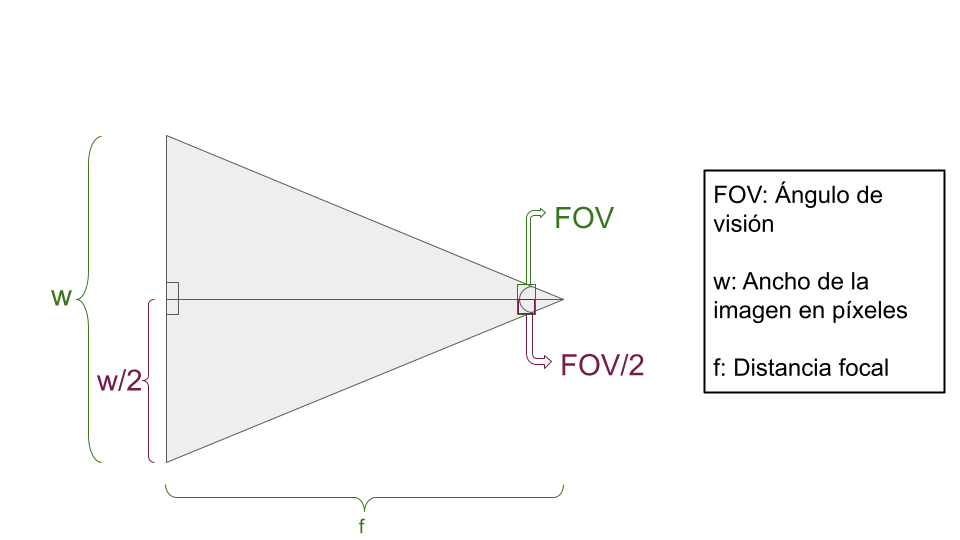
\includegraphics[scale=0.4]{Imágenes/semana2-triangulos.png}
    \caption{Relación entre FOV, ancho de la imagen y distancia focal}
    \label{fig:semana2FOV}
\end{figure}

Como se puede observar, la tangente de $\frac{FOV}{2}$ es igual a $\frac{w/2}{f}$ por la definición de tangente\footnote{En triángulos rectángulos, la tangente es la razón entre el cateto opuesto y el adyacente}. De este modo, se obtiene la fórmula:

$$tan\left(\frac{FOV_{horizontal}}{2}\right) = \frac{w/2}{f}$$

Si se quiere calcular el FOV vertical, bastaría con cambiar el ancho de la imagen por el largo de esta. Serviría la fórmula anterior, siendo $w$ la altura en vez del ancho de la imagen.

\subsubsection*{Cálculos}

Ya se tiene la \textbf{distancia focal}, que se calculó en el ejercicio \ref{sec:hands}, en el caso de mi cámara es \textbf{738 píxeles}. Para despejar la fórmula es necesario indicar que la cámara toma fotografías de un ancho de 640 píxeles (w).

$$tan\left(\frac{FOV}{2}\right) = \frac{w/2}{f} \rightarrow FOV = arctan\left(\frac{w/2}{f}\right)*2 = arctan\left(\frac{640/2}{738}\right)*2 = 46.88\degree$$

Se obtiene un \textbf{FOV horizontal} de \textbf{46.88 grados}.

Ahora, se calculará el vertical (las fotografías tomadas por la cámara tienen un alto de 360 píxeles):

$$tan\left(\frac{FOV}{2}\right) = \frac{w/2}{f} \rightarrow FOV = arctan\left(\frac{w/2}{f}\right)*2 = arctan\left(\frac{360/2}{738}\right)*2 = 27.4\degree$$

Se obtiene un \textbf{FOV vertical} de \textbf{27.4 grados}.

\subsection*{Ángulo entre 2 puntos}

Para calcular el ángulo que forman los rayos ópticos correspondientes  a dos píxeles marcados con el ratón, se debe de tener en cuenta la imagen \ref{fig:angulo-entre-puntos}, perteneciente a los apuntes de la asignatura.


\begin{figure} [h]
    \centering
    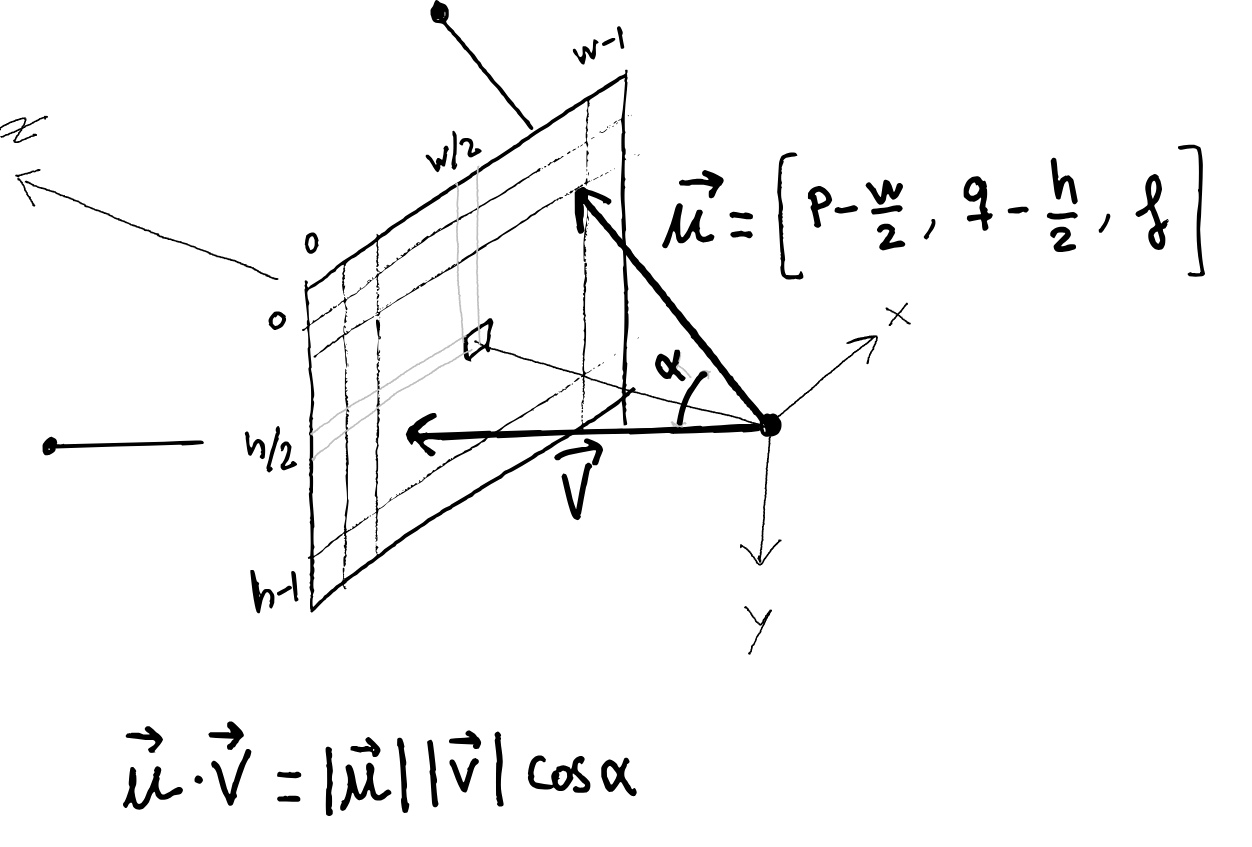
\includegraphics[width=0.5\linewidth]{Imágenes/Imagen-angulo-puntos-material-asignatura.png}
    \caption{Ángulo entre puntos de la imagen (pertenece a \href{https://raw.githubusercontent.com/albertoruiz/umucv/master/images/demos/anglepixs.svg}{los apuntes de la asignatura})}
    \label{fig:angulo-entre-puntos}
\end{figure}
Como se puede observar en la imagen, si se tiene la distancia focal, se puede obtener el vector que va hasta un punto de la imagen. Cogiendo el inicio del vector como (0,0,0), se tiene:

\begin{itemize}
    \item El desplazamiento en x: Es la coordenada x del punto en la imagen (en píxeles) menos la mitad del ancho de la imagen (en píxeles) ya que el inicio del vector se encuentra en el centro. 
    \item El desplazamiento en y: Se calcula de forma similar al anterior, con la coordenada en y del punto en la imagen menos la mitad del alto de la imagen (el inicio del vector se encuentra en el centro).
    \item El desplazamiento en z: Es la distancia focal (en píxeles) de la imagen. 
\end{itemize}

Una vez obtenidos los dos vectores de dos puntos, se puede calcular el ángulo que estos forman con la fórmula siguiente:

\[
\cos(\alpha) = \frac{\vec{u} \cdot \vec{v}}{|\vec{u}| |\vec{v}|} \rightarrow \alpha = \arccos{\frac{\vec{u} \cdot \vec{v}}{|\vec{u}| |\vec{v}|}}
\]

Y con todo esto, se obtiene el ángulo ($\alpha$) entre los vectores (los rayos ópticos correspondientes a dos píxeles marcados con el ratón).

\subsubsection*{Código}

Se ha modificado el código de \textit{medidor.py} para añadir una función que calcula el ángulo entre los vectores dados sus puntos en la imagen. Se ha almacenado en variables la distancia focal, el alto y el ancho de la cámara (en píxeles) de forma que se pueda calcular el ángulo de la forma anteriormente explicada.

Después, se ha añadido al texto mostrando la distancia entre los puntos, los ángulos que estos forman.

\subsection*{Cámara usada}

Al utilizar la distancia focal y el FOV de la cámara para realizar el ejercicio, es importante indicar la cámara que se utiliza. Se ha cogido como referencia la cámara de un portátil Acer Aspire 3.

\subsection*{Jupyter notebook}

\textit{Utiliza el script para encontrar mediante una construcción geométrica la posición aproximada en un mapa desde la que se ha tomado una imagen en la que se ven algunos puntos característicos.}

Se ha realizado un notebook en el que se puede observar el cálculo de la posición desde la que se ha tomado una fotografía dados dos puntos característicos. Este notebook se encuentra en \textit{ejercicioMAPA.ipynb}.

Las imágenes que se encuentran en la carpeta \textit{img} son imágenes usadas en el notebook.

\subsection*{Bibliografía usada}
\href{https://github.com/albertoruiz/umucv/blob/master/notebooks/imagen.ipynb}{Material de la asignatura}

\href{https://www.sony.es/electronics/support/articles/00267921}{Entender qué es la distancia focal}

\href{https://www.blogdelfotografo.com/tipos-caracteristicas-ventajas-sensores-camaras-fotos/}{Entender qué es un sensor}

\href{https://www.superprof.es/apuntes/escolar/matematicas/geometria/basica/triangulos-en-posicion-de-thales.html}{Teorema de Thales}

\href{https://numpy.org/doc/stable/reference/generated/numpy.dot.html}{numpy dot}

\href{https://numpy.org/doc/stable/reference/generated/numpy.linalg.norm.html#numpy-linalg-norm}{numpy norm}

\href{https://numpy.org/doc/stable/reference/generated/numpy.arccos.html}{numpy arccos}

\href{https://numpy.org/doc/stable/reference/generated/numpy.degrees.html}{numpy degrees}

\href{https://numpy.org/doc/stable/reference/generated/numpy.array.html}{numpy array}
\end{document}